% Beziehungen zwischen den Klassen der polynomiellen Hierarchie.
% Adaptiert nach Rapberger (2023), Abb. 6.1, S. 116.
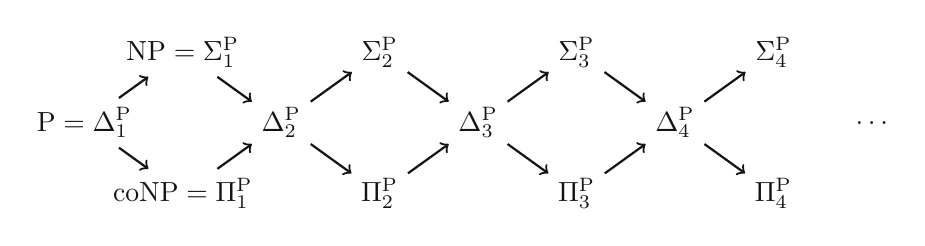
\begin{tikzpicture}[
    ph class/.style={
        font=\sffamily,
        text=black!92
    },
    ph inclusion/.style={
        ->,
        thick,
        draw=black!92
    }
]
    % Mittlere Ebene (Delta-Klassen)
    \node[ph class] (delta1) at (0,0)
        {$\mathrm{P} = \Delta_{1}^{\mathrm{P}}$};
    \node[ph class] (delta2) at (2.5,0)
        {$\Delta_{2}^{\mathrm{P}}$};
    \node[ph class] (delta3) at (5,0)
        {$\Delta_{3}^{\mathrm{P}}$};
    \node[ph class] (delta4) at (7.5,0)
        {$\Delta_{4}^{\mathrm{P}}$};
    \node[ph class] at (10,0) {$\ldots$};

    % Obere und untere Ebenen (Sigma- und Pi-Klassen)
    \node[ph class] (sigma1) at (1.25,0.9)
        {$\mathrm{NP} = \Sigma_{1}^{\mathrm{P}}$};
    \node[ph class] (pi1) at (1.25,-0.9)
        {$\mathrm{coNP} = \Pi_{1}^{\mathrm{P}}$};

    \foreach \level/\xpos in {2/3.75,3/6.25,4/8.75} {
        \node[ph class] (sigma\level) at (\xpos,0.9)
            {$\Sigma_{\level}^{\mathrm{P}}$};
        \node[ph class] (pi\level) at (\xpos,-0.9)
            {$\Pi_{\level}^{\mathrm{P}}$};
    }

    % Pfeile bezeichnen Mengeninklusionen; alle verlaufen von links nach rechts.
    \foreach \level in {1,...,4} {
        \draw[ph inclusion] (delta\level) -- (sigma\level);
        \draw[ph inclusion] (delta\level) -- (pi\level);
    }
    \foreach \level/\nextlevel in {1/2,2/3,3/4} {
        \draw[ph inclusion] (sigma\level) -- (delta\nextlevel);
        \draw[ph inclusion] (pi\level) -- (delta\nextlevel);
    }
\end{tikzpicture}
